%!TEX program = xelatex
\documentclass[color=blue,mathpazo,titlestyle=hang,11pt]{elegantbook}

\usepackage{indentfirst}


\author{LMin}
\email{luomin5417@gmail.com}
\zhtitle{自制脚本语言}
\zhend{笔记}
\entitle{Homemada Script Luaguage}
\enend{Note}
\version{0.1}
\myquote{There is no good end for the fuck thieves country.}
\logo{logo.pdf}
\cover{cover.pdf}

%green color
   \definecolor{main1}{RGB}{0,120,2}
   \definecolor{seco1}{RGB}{230,90,7}
   \definecolor{thid1}{RGB}{0,160,152}
%cyan color
   \definecolor{main2}{RGB}{0,175,152}
   \definecolor{seco2}{RGB}{239,126,30}
   \definecolor{thid2}{RGB}{120,8,13}
%blue color
   \definecolor{main3}{RGB}{20,50,104}
   \definecolor{seco3}{RGB}{180,50,131}
   \definecolor{thid3}{RGB}{7,127,128}

\usepackage{makecell}
\usepackage{lipsum}
\usepackage{texnames}
\usepackage{float}


\begin{document}
\maketitle
\tableofcontents
\mainmatter

\chapter{语言处理器基本概}

\begin{center}
学而不思则罔,思而不学则怠!
\end{center}

\begin{flushright}
---孔子    
\end{flushright}

\section{机器语言与汇编语言}
本节主要介绍了机器语言与汇编语言:
\begin{itemize}
    \item 机器语言是可以由机器直接解释执行的语言,一般才用二进制形式\cite{complete}。
    \item 汇编语言一般是相对于机器语言更易理解的语言,但是又因不同的体系结构不同具有不
    同的指令集。
\end{itemize} 


\section{解释器与编译器}
本节主要介绍了解释器和编译器的区别:
\begin{itemize}
    \item 解释器根据程序中的算法执行运算。
    \item 编译器将某种语言写成的程序转换为另一种语言的程序。
\end{itemize}    
    
\section{开发语言处理器}
本节主要介绍语言处理器,综合了解释器和编译器的优点。

\section{语言处理器结构与本书框架}
语言处理器的基本结构,如图1.1所示,画出了语言处理器的基本处理结构,源程序通过词法分析进行
单词排列,然后经过语法分析生成一个抽象语法树,然后根据是编译器还是解释器执行不同的步骤,
如果是编译器则直接生成机器语言,如果是解释器则一边分析抽象语法树,一边输出执行结果。
\begin{figure}[hbtp]
\centering
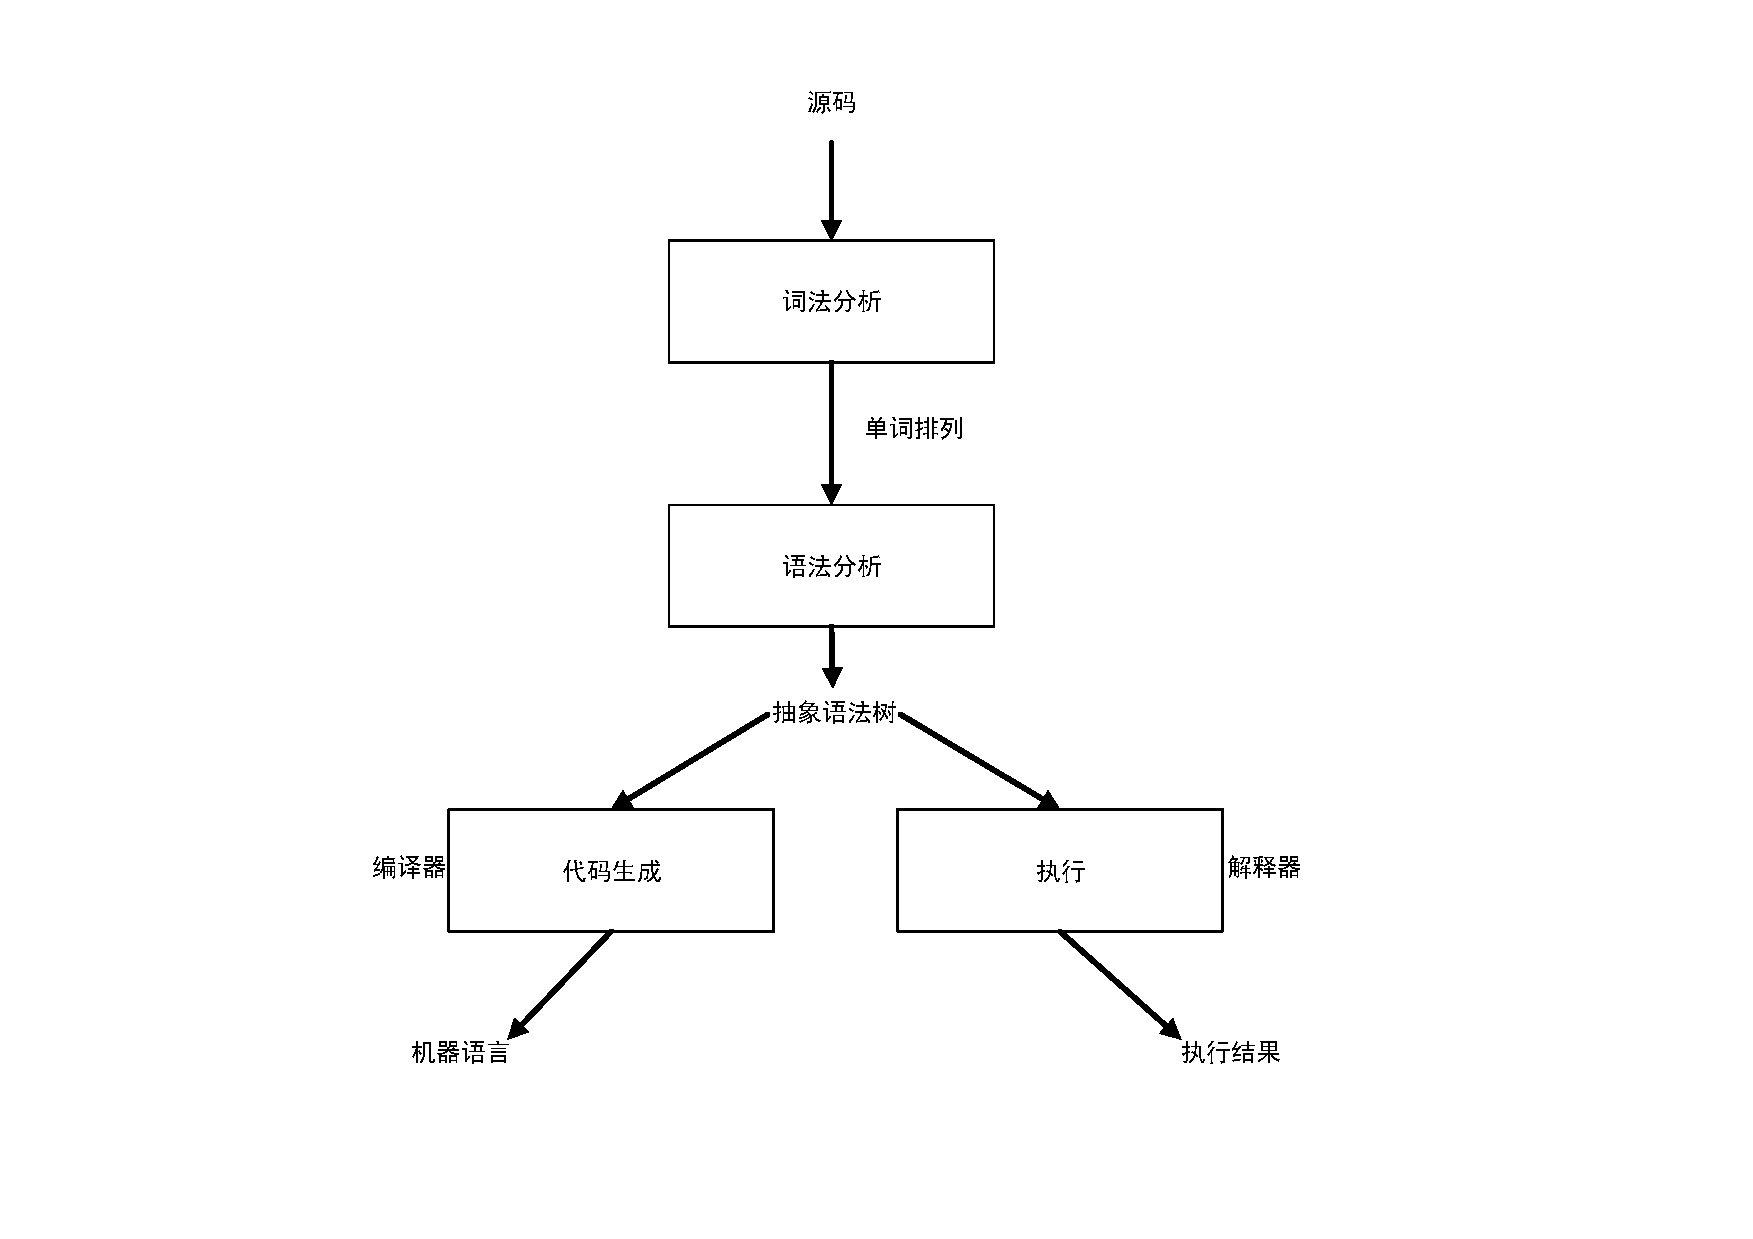
\includegraphics[width=1.0\textwidth]{construction.pdf}
\caption{语言处理器结构}
\end{figure}


无论是编译器还是解释器的结构都是大同小异的,第一步都是要先进行词法分析,由一长串字符分解
成为多个更小的字符串单元,然后执行语法分析,把单词排列成为抽象语法树,到此解释器与编译器
的行为都是一致的,在这之后编译器将转换为另外的语言,而解释器则将一边分析语法树一边执行。
\chapter{设计脚本语言}

\begin{flushleft}
故不登高山,不知天之高也;不临深溪,不知地之厚也;不闻先王之遗言,不知学问之大也。
\end{flushleft}

\begin{flushright}
---荀子   
\end{flushright}

\section{麻雀虽小五脏俱全}

设计脚本语言的基本元素如图2.1所示:

\begin{figure}[hbtp]
\centering
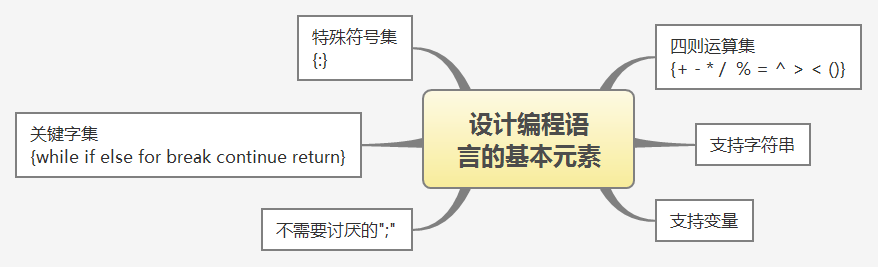
\includegraphics[width=1.0\textwidth]{pl.png}
\caption{脚本语言构成要素}
\end{figure}

只有具备这些基本元素才能算为一个完备的脚本语言,暂定这些基本元素,后期在有需要再进行进一
步的修改:
\begin{itemize}
	\item 支持四则运算
	\item 支持字符串
	\item 支持变量
	\item 一些其它特性,如不支持‘;’
	\item 支持基本逻辑关键字
\end{itemize}


\chapter{Linux Camera驱动框架}

\begin{center}
为往圣继绝学,为万世开太平!
\end{center}

\begin{flushright}
---张载  
\end{flushright}

\section{矩阵和向量}
\lipsum[3]
考虑如下的随机动态规划问题
\begin{align*}
&\max(\min)\quad \mathbb{E}\int_{t_0}^{t_1}f(t,x,u)\,dt\\
&\quad\mbox{s.t.} \quad dx=g(t,x,u)dt+\sigma(t,x,u)dz\\
&\quad \hspace{2.em} k(0)=k_0\;\text{given}
\end{align*}

where $z$ is stochastic process or white noise or wiener process.

\begin{newdef}[Wiener Process]
If $z$ is wiener process, then for any partition $t_0,t_1,t_2,\ldots$ of time interval, the random variables $z(t_1)-z(t_0),z(t_2)-z(t_1),\ldots$ are independently and normally distributed with zero means and variance $t_1-t_0,t_2-t_1,\ldots$
\end{newdef}

\lipsum[5]

\begin{example}
$E$ and $F$ be two events such that $\mbf{P}(E)=\mbf{P}(F)=1/2$, and $\mbf{P}(E\cap F)=1/3$, let $\mathscr{F}=\sigma(Y)$,  $X$ and $Y$ be the indicate function of $E$ and $F$ respectively. How to compute $\mathbb{E}[ X\mid \mathscr{F} ]$?
\end{example}
\lipsum[4]
\begin{exercise}
let $S=l^\infty=\big\{(x_n)\mid \exists\, M \text{ such that } \forall n, |x_n|\leq M,x_n\in \mathbb{R}\big\}$, $\rho_{\infty}(x,y)=\sup\limits_{n\geq 1}|x_n-y_n|$, show that $\big(l^\infty,\rho_{\infty}\big)$ is complete.
\end{exercise}

\begin{newthem}[勾股定理]
勾股定理的数学表达(Expression)为
\[a^2+b^2=c^2\]
其中$a,b$为直角三角形的两条直角边长,$c$为直角三角形斜边长。
\end{newthem}

\begin{note}
在本模板中,引理(lemma),推论(corollary )的样式和定理的样式一致,包括颜色,仅仅只有计数器的设置不一样。在这个例稿中,我们将不给出引理推论的例子。
\end{note}


\lipsum[4]

\begin{newprop}[最优性原理]
如果$u^*$在$[s,T]$上为最优解,则$u^*$在$[s,T]$任意子区间都是最优解,假设区间为$[t_0,t_1]$的最优解为$u^*$,则$u(t_0)=u^{*}(t_0)$,即初始条件必须还是在$u^*$上。
\end{newprop}

\lipsum[5-6]
\begin{newcorol}
假设$V(\cdot,\cdot)$为值函数,则跟据最大值原理,有如下推论
\[
V(k,z)=\max\Big\{u\big(zf(k)-y\big)+\beta \mathbb{E}V(y,z^\prime)\Big\}
\]
\end{newcorol}

\begin{newproof}
因为 $y^*=\alpha\beta z k^\alpha$,$V(k,z)=\alpha/1-\alpha\beta\ln k_0+1/1-\alpha\beta \ln z_0+\Delta$。
\begin{align*}
\text{右边}&=\Big\{u\big(zf(k)-y\big)+\beta \mathbb{E}V(y,z^\prime)\Big\}\\
&=\ln(zk^\alpha-\alpha\beta zk^\alpha)+\beta\mathbb{E}\Big[\frac{\alpha}{1-\alpha\beta}\ln y+\frac{1}{1-\alpha\beta}\ln z^\prime+\Delta\Big]\\
&=\ln(1-\alpha\beta)zk^\alpha+\beta\Big\{\mathbb{E}\big[\frac{\alpha}{1-\alpha\beta}\ln \alpha\beta z k^\alpha\big]+\frac{1}{1-\alpha\beta}\mathbb{E}[\ln z^\prime]+\Delta\Big\}
\end{align*}
利用$\mathbb{E}[\ln z^\prime]=0$,并将对数展开得
\begin{align*}
\text{右边}&=\ln (1-\alpha\beta)+\ln z+\alpha\ln k+\frac{\alpha\beta}{1-\alpha\beta}\big[\ln \alpha\beta+\ln z+\alpha\ln k\big]+\frac{\beta}{1-\alpha\beta}\mu+\beta \Delta\\
&=\frac{\alpha}{1-\alpha\beta}\ln k+\frac{1}{1-\alpha\beta}\ln z+\Delta
\end{align*}
所以$\text{左边}=\text{右边}$,证毕。
\end{newproof}



\begin{property}
Properties of Cauchy Sequence
\begin{enumerate}\parskip=0pt \itemsep=0pt
\item $\{x_k\}$ is cauchy sequence then $\{x_k^i\}$ is cauchy sequence.
\item $x_k\in \mathbb{R}^n$, $\rho(x,y)$ is Euclidean, then cauchy is equivalent to convergent, $(\mathbb{R}^n,\rho)$ metric space is complete.
\end{enumerate}
\end{property}


\lipsum[7]

\begin{custom}{Application}
This is one example of the custom environment, the key word is given by the option of custom environment.
\end{custom}


\lipsum[6]
\begin{newdef}[Contraction mapping]
$(S,\rho)$ is the metric space, $T: S\to S$, If there exists $\alpha\in(0,1)$ such that for any $x$ and $y\in S$, the distance
\begin{equation}
\rho(Tx,Ty)\leq \alpha\rho(x,y)
\end{equation}
Then $T$ is a {\color{main} contraction mapping}.
\end{newdef}

\begin{remark}
\begin{enumerate}
\parskip=0pt \itemsep=0pt
\item $T:S\to S$, where $S$ is a metric space, if  for any $x,y\in S$, $\rho(Tx,Ty)<\rho(x,y)$ is not contraction mapping.
\item Contraction mapping is continuous map.
\end{enumerate}
\end{remark}


\begin{conclusion}
看到一则小幽默,是这样说的:{\color{main} 别人都关心你飞的有多高,只有我关心你的翅膀好不好吃!}说多了都是泪啊!
\end{conclusion}

\section{加法和标量乘法}

\section{矩阵向量乘法}

\section{矩阵乘法}

\section{矩阵乘法特征}

\section{逆和转制}
\chapter{全志A83t Camera开发}
\begin{center}
纸上得来终觉浅,绝知此事要躬行。
\end{center}

\begin{flushright}
---傅玄
\end{flushright}

\section{总线与硬件接口}

根据全志官方提供的《A83t\_User\_Manual》和《A83t\-Datasheet》两个文档,可以知道A83t支持MIPI-CSI
总线和CSI总线,且A83t内部支持ISP,A83t体系架构图如图4.1所示。

\begin{figure}[!hbtp]
\centering
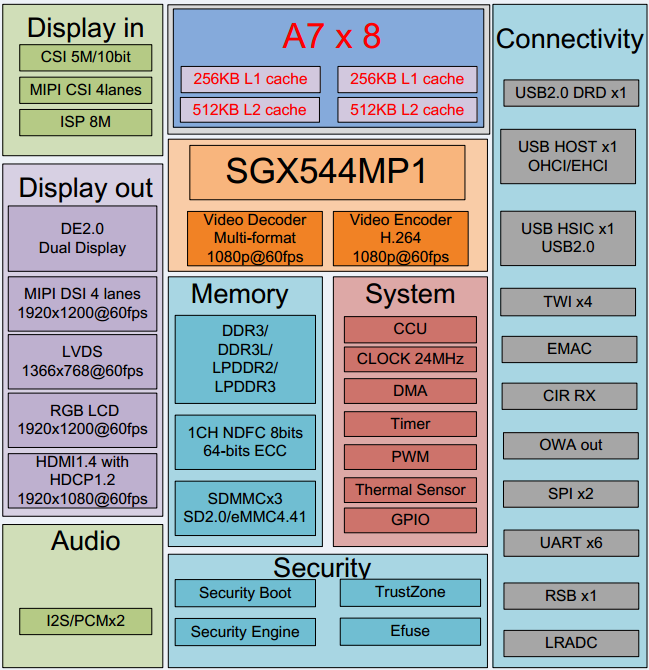
\includegraphics[width=0.8\textwidth]{Achitechture.png}
\caption{A83t体系架构\label{figur:A83t_Achitechture}}
\end{figure}

CSI接口的特性如图4.2,
\begin{figure}[H]
\centering
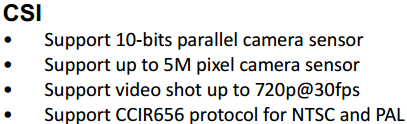
\includegraphics[width=0.8\textwidth]{CSI_feature.png}
\caption{CSI接口特性\label{figur:CSI_feature}}
\end{figure}

MIPI-CSI接口的特性如图4.3,
\begin{figure}[H]
\centering
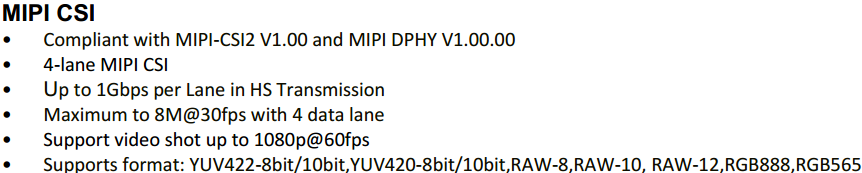
\includegraphics[width=0.8\textwidth]{MIPI-CSI_feature.png}
\caption{MIPI-CSI接口特性\label{figur:MIPI-CSI_feature}}
\end{figure}


\section{硬件原理图}
在调试的开发板上采用的是gc2145+gc0329连接到A83t的CSI0接口,gc2145器件原理图如图4.4所示,
\begin{figure}[H]
\centering
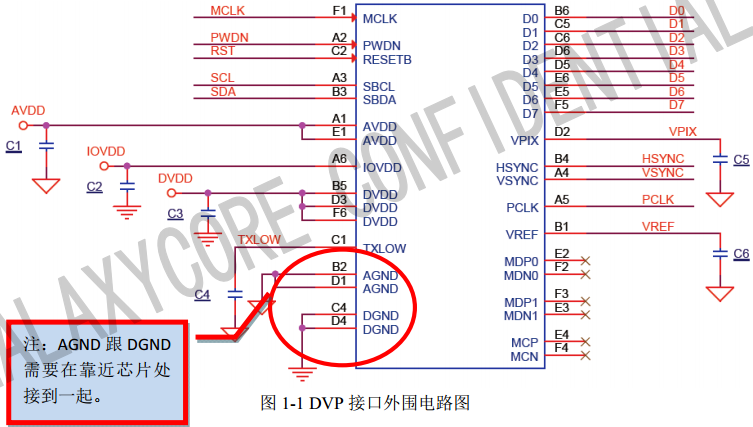
\includegraphics[width=0.8\textwidth]{GC2145.png}
\caption{GC2145器件原理图\label{figur:GC2145}}
\end{figure}
\section{驱动源码}

\section{内核与驱动配置}
调试camera需要配置内核与sysconfig.fex文件,内核配置如图4.6所示。
\begin{figure}[H]
\centering
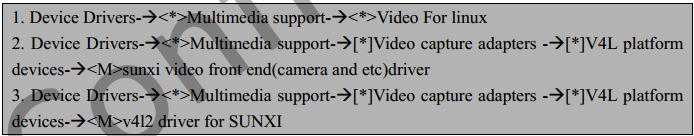
\includegraphics[width=0.8\textwidth]{menuconfig.png}
\caption{make menuconfig配置\label{figur:menuconfig}}
\end{figure}

除了基本的内核对camera的支持,还需要修改内核Makefile添加爱gc2145驱动的编译,修改文件路径:
linux-3.4/drivers/media/video/sunxi-vfe/device/Makefile,修改内容如图4.7所示,在24行添加了gc2145sensor模组的驱动编译,
\begin{figure}[H]
\centering
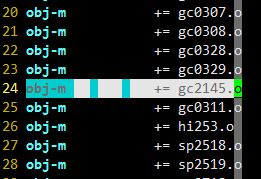
\includegraphics[width=0.8\textwidth]{gc2145_driver.png}
\caption{添加GC2145驱动\label{figur:gc2145_driver}}
\end{figure}

完成内核配置之后还需要对android系统进行配置,让android系统在启动时加载对应的驱动模块,对应的修改目录:
android/device/softwinner/octopus-f1/init.sun8i.rc,修改内容如图4.8所示,添加了加载gc2145.ko模块,去掉了ov5640模块的加载。
\begin{figure}[H]
\centering
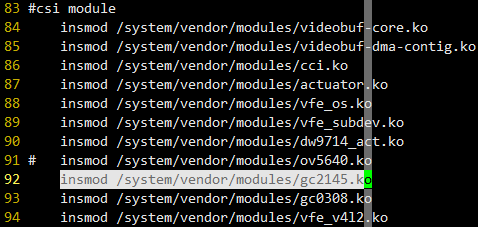
\includegraphics[width=0.8\textwidth]{android_init.png}
\caption{加载GC2145驱动\label{figur:android_init}}
\end{figure}

\section{调试问题记录}
将调试中遇到的一些问题记录如下:

\begin{enumerate}[1)]
\item \textbf{将sysconfig.fex文件配置好之后,编译固件下载运行,在linux加载时出现卡住无法启动的问题。}
\begin{figure}[H]
\centering
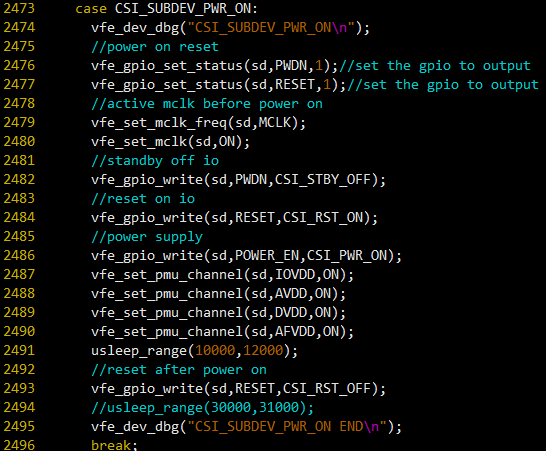
\includegraphics[width=0.8\textwidth]{bug_code01.png}
\caption{定位代码\label{figur:bug_code01}}
\end{figure}

解决方法:在各个驱动里面添加打印,定位具体是什么位置导致了CPU死掉,初步判断是有空指针之类的问题,但是内核栈没有更多的信息打印出来。
还想到一个办法,便是通过将android中设置的自动加载camera各个驱动,换成手动加载驱动,看看是如何挂掉的。
添加打印后和换成手动加载驱动之后定位到挂掉的代码位置,代码路径linux-3.4/drivers/media/video/sunxi-vfe/device/gc2145.c,
如图4.8所示,最后定位到了vfe\_set\_pmu\_channel(sd, IOVDD, ON)这一句,原来是在sys\_config.fex中iovdd-csi位置设置错误,放到了
aldo2下面,aldo2是控制sdram和pll的电源。

完成电源配置之后,摄像头便可以正常启动了,此时的sys\_config.fex的电源分配如图4.9所示,将iovdd-csi分配到了axp81x\_dldo3,将
dvdd-csi-18分配在了axp81x\_eldo1,avdd-csi分配在了axp81x\_dldo4。
\begin{figure}[htbp]
\centering
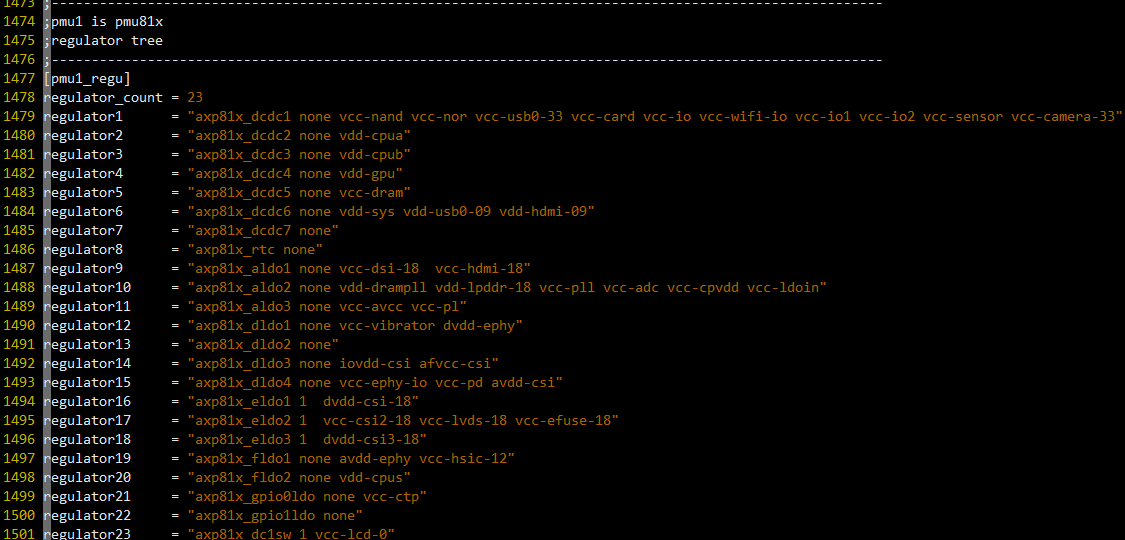
\includegraphics[width=0.8\textwidth]{sys_config0.png}
\caption{sys\_config电源分配\label{figur:sys_config0}}
\end{figure}

iovdd是摄像头模块io接口电源,avdd是摄像头模块模拟电路电源,dvdd是摄像头模块数字电路电源,具体电源配置电压如图4.10所示,
\begin{figure}[htbp]
\centering
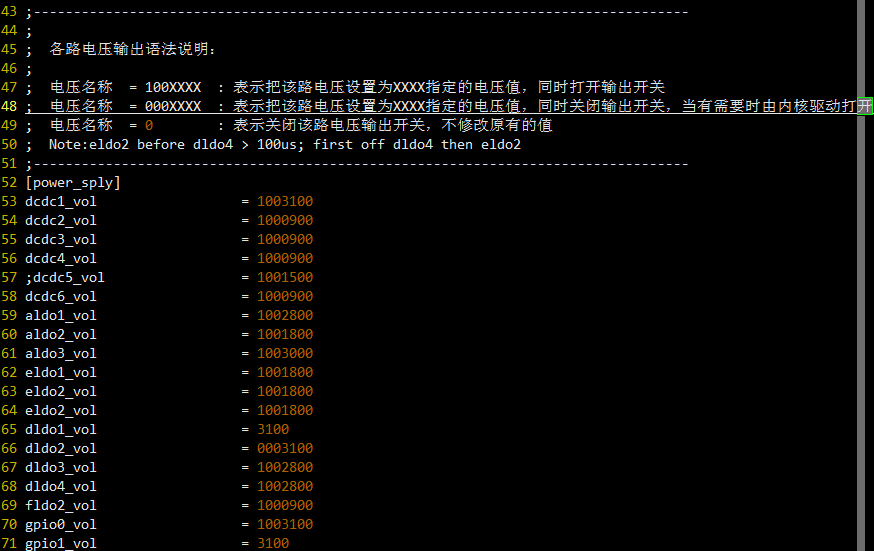
\includegraphics[width=0.8\textwidth]{sys_config1.png}
\caption{sys\_config电源电压配置\label{figur:sys_config1}}
\end{figure}



\item \textbf{驱动挂死}

解决方法:

\end{enumerate}

    
\section{总结}
\chapter{多变量线性回归}

\section{多功能}

\section{多元梯度下降法}

\section{多元梯度下降法演练I-特征缩放}

\section{多元梯度下降法演练II-学习率}

\section{特征和多项式回归}

\section{正规方程(区别于迭代方法的直接解决)}

\section{正规方程在矩阵不可逆情况下的解决方法}

\section{完成并提交编程作业}
%\chapter{Octave/Matlab教程}

\section{基本操作}

\section{移动数据}

\section{计算数据}

\section{数据绘制}

\section{控制语句:for, while, if语句}

\section{矢量}

\section{本章课程总结}
%\chapter{Logistic回归}

\section{分类}

\section{假设陈述}

\section{决策界限}

\section{代价函数}

\section{简化代价函数与梯度下降}

\section{高级优化}

\section{多元分类:一对多}

\section{本章课程总结}
%
\chapter{正则化}

\section{过拟合问题}

\section{代价函数}

\section{线性回归的正则化}

\section{Logistic回归的正则化}

\bibliographystyle{ieeetr}
\bibliography{reference}
\addcontentsline{toc}{chapter}{参考文献}

\end{document}